\sloppy
\section{1. Установка и подготовка}

Цель работы в том, чтобы поднять ансамбль из трех серверов ZooKeeper,
проверить роли серверов, работу при потере одного и двух серверов и
эфемерный узел, а затем сделать отказоустойчивым координатор расчета пар
навыков из третьей работы. Вариант 9, программист, разработчик на мобильных
платформах.

Работа выполнена 10 ноября 2026 года на macOS с Docker Desktop. Три сервера
подняты в Docker из официального образа zookeeper:3.9.6-jre-17. В образе
ZooKeeper 3.9.6 распакован в папку /apache-zookeeper-3.9.6-bin, там же есть
Java 17, переменная JAVA\_HOME указывает на /opt/java/openjdk, поэтому
отдельно на компьютер Java 17 не ставится. Каждый
контейнер запускает сервер штатной командой zkServer.sh start-foreground.

\begin{figure}[H]
\centering
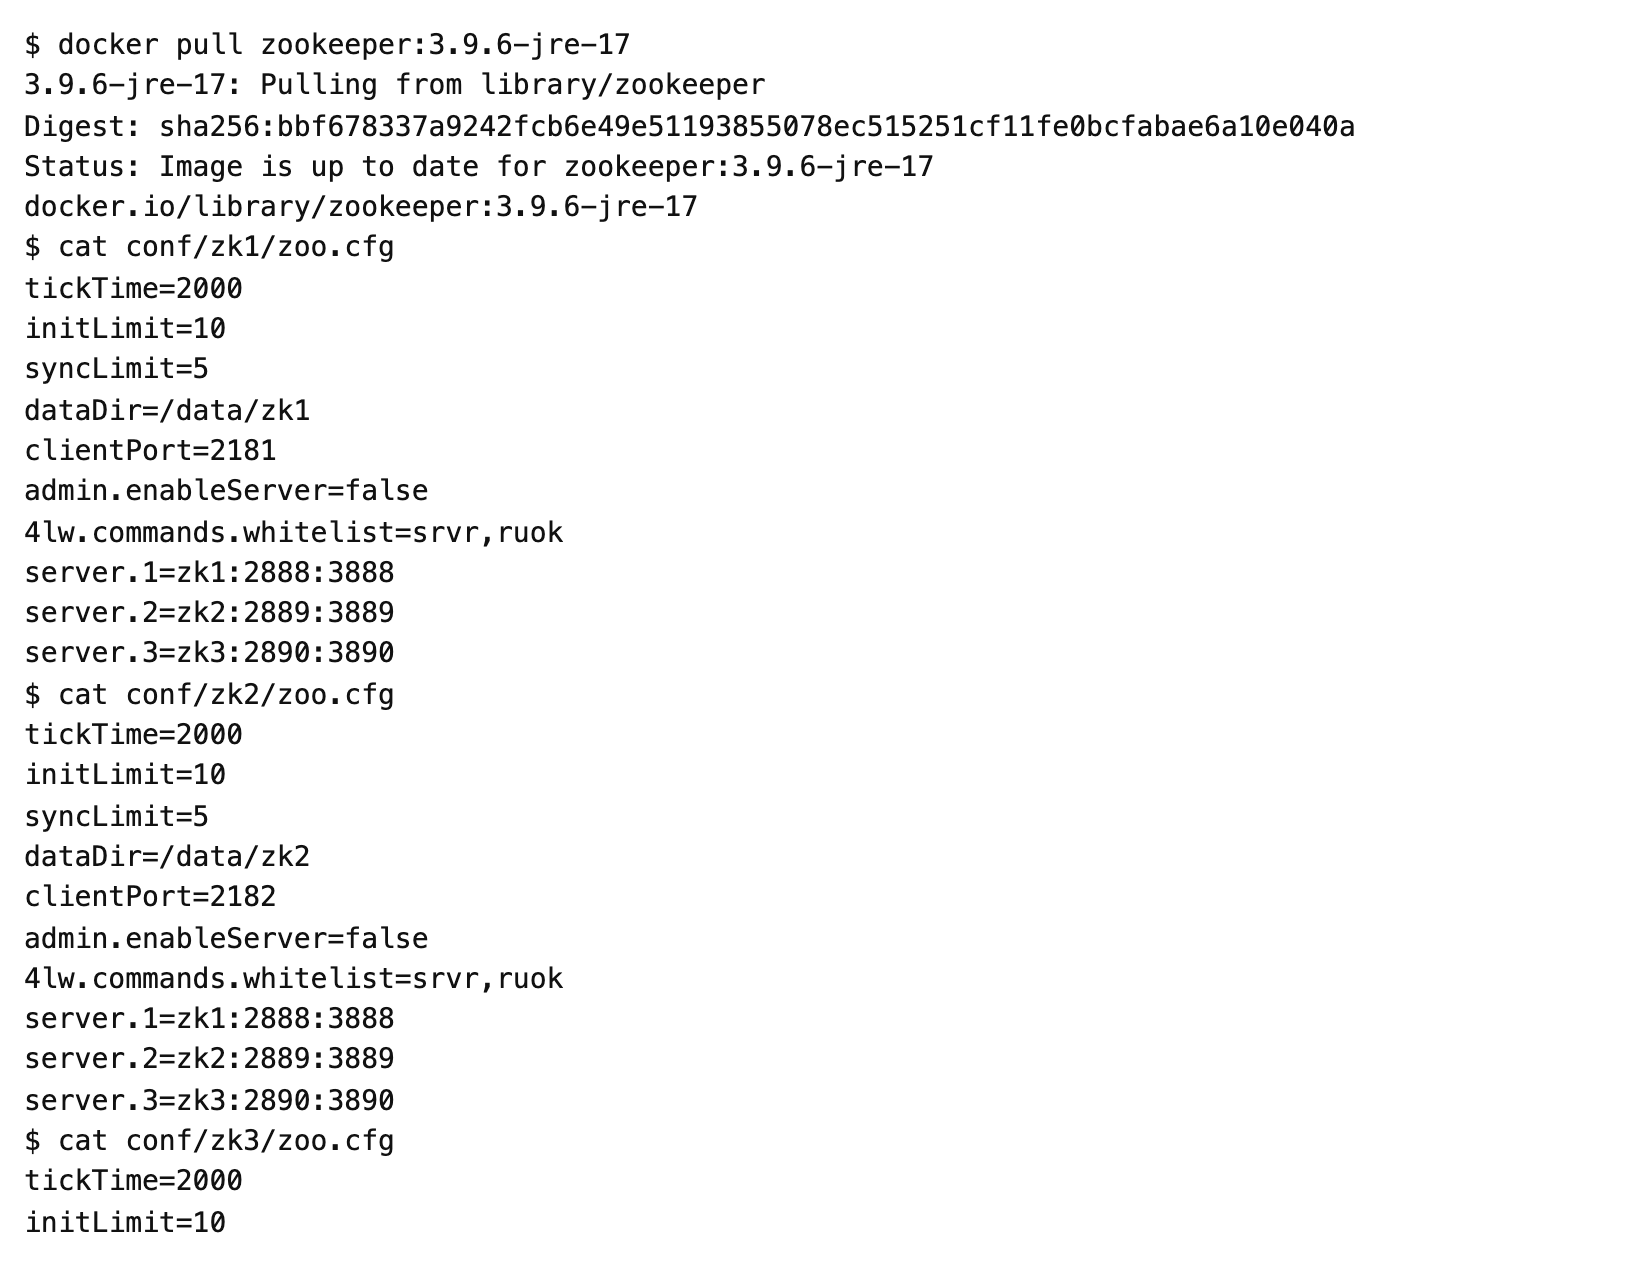
\includegraphics[width=0.85\textwidth,height=0.78\textheight,keepaspectratio]{../screenshots/01_setup_1.png}
\caption{Образ, конфигурации, файлы myid, запуск ансамбля и версия Java, часть 1 из 3}
\end{figure}

\begin{figure}[H]
\centering
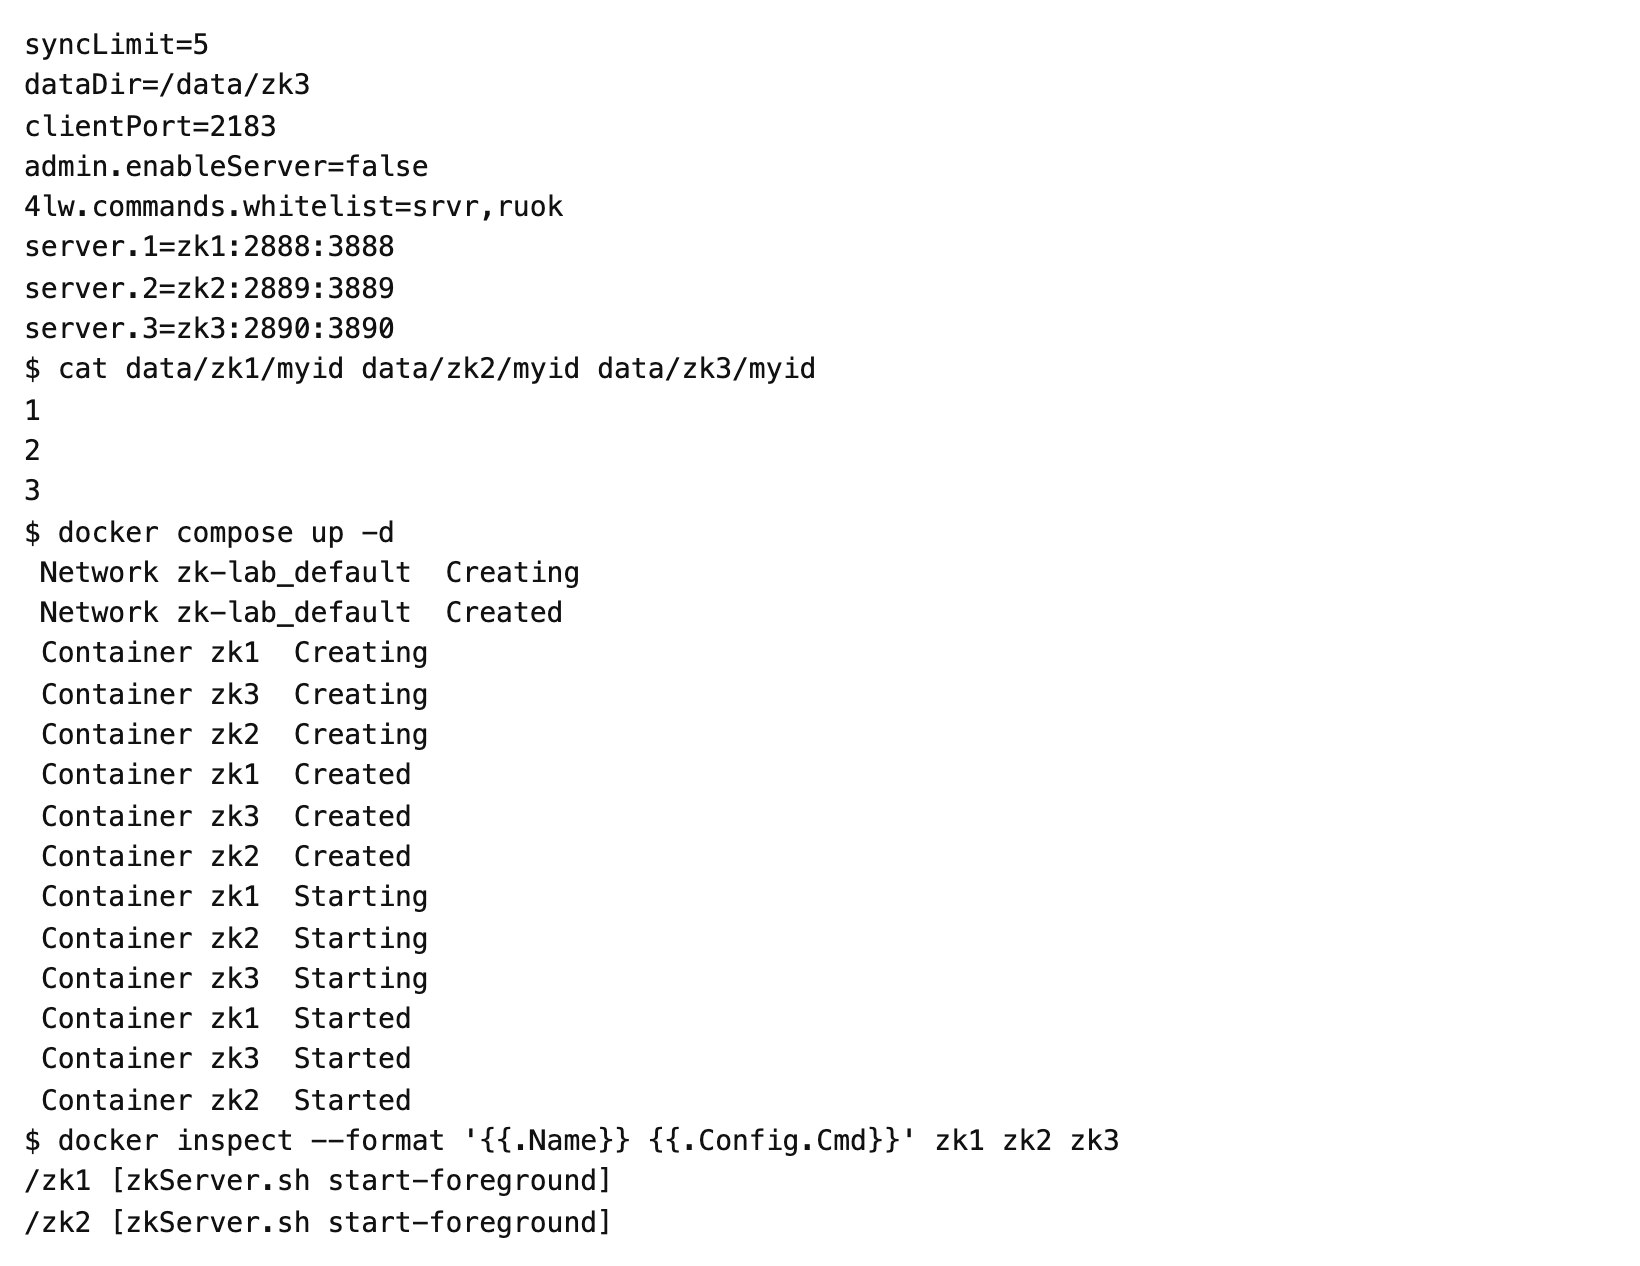
\includegraphics[width=0.85\textwidth,height=0.78\textheight,keepaspectratio]{../screenshots/01_setup_2.png}
\caption{Образ, конфигурации, файлы myid, запуск ансамбля и версия Java, часть 2 из 3}
\end{figure}

\begin{figure}[H]
\centering
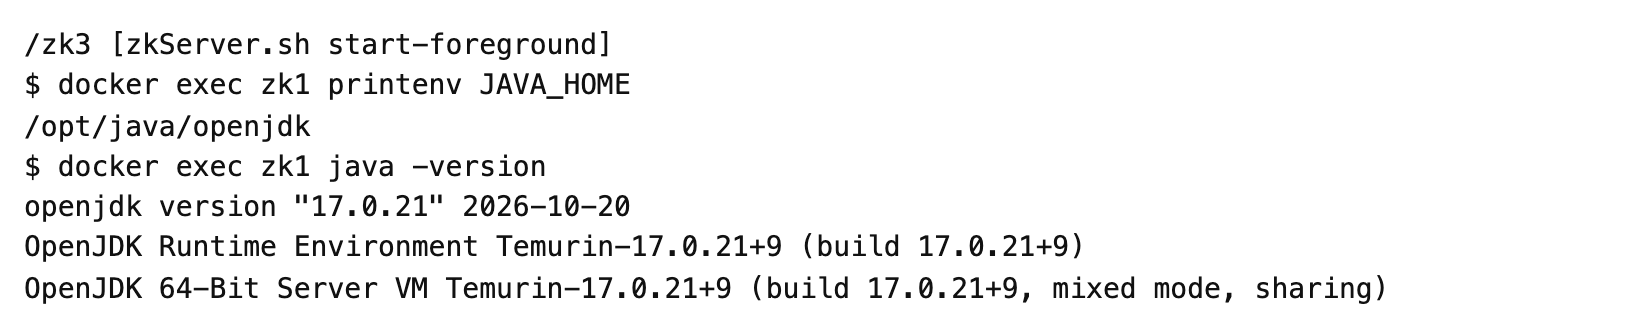
\includegraphics[width=0.85\textwidth,height=0.78\textheight,keepaspectratio]{../screenshots/01_setup_3.png}
\caption{Образ, конфигурации, файлы myid, запуск ансамбля и версия Java, часть 3 из 3}
\end{figure}

\section{2. Ансамбль ZooKeeper}

У каждого сервера своя конфигурация conf/zoo.cfg. Строки участников
server.1, server.2 и server.3 у всех одинаковые. Клиентские порты разные,
2181, 2182 и 2183, у каждого сервера свои порты обмена с лидером и выборов,
2888 и 3888, 2889 и 3889, 2890 и 3890. Папка dataDir тоже своя, /data/zk1,
/data/zk2 и /data/zk3, она смонтирована из локальной папки data. В каждой
dataDir лежит файл myid с номером 1, 2 или 3, по нему сервер находит свою
строку server.N.

\begin{code}
tickTime=2000
initLimit=10
syncLimit=5
dataDir=/data/zk2
clientPort=2182
server.1=zk1:2888:3888
server.2=zk2:2889:3889
server.3=zk3:2890:3890
\end{code}

После запуска команда zkServer.sh status показала, что zk3 стал лидером, а
zk1 и zk2 последователями.

\begin{figure}[H]
\centering
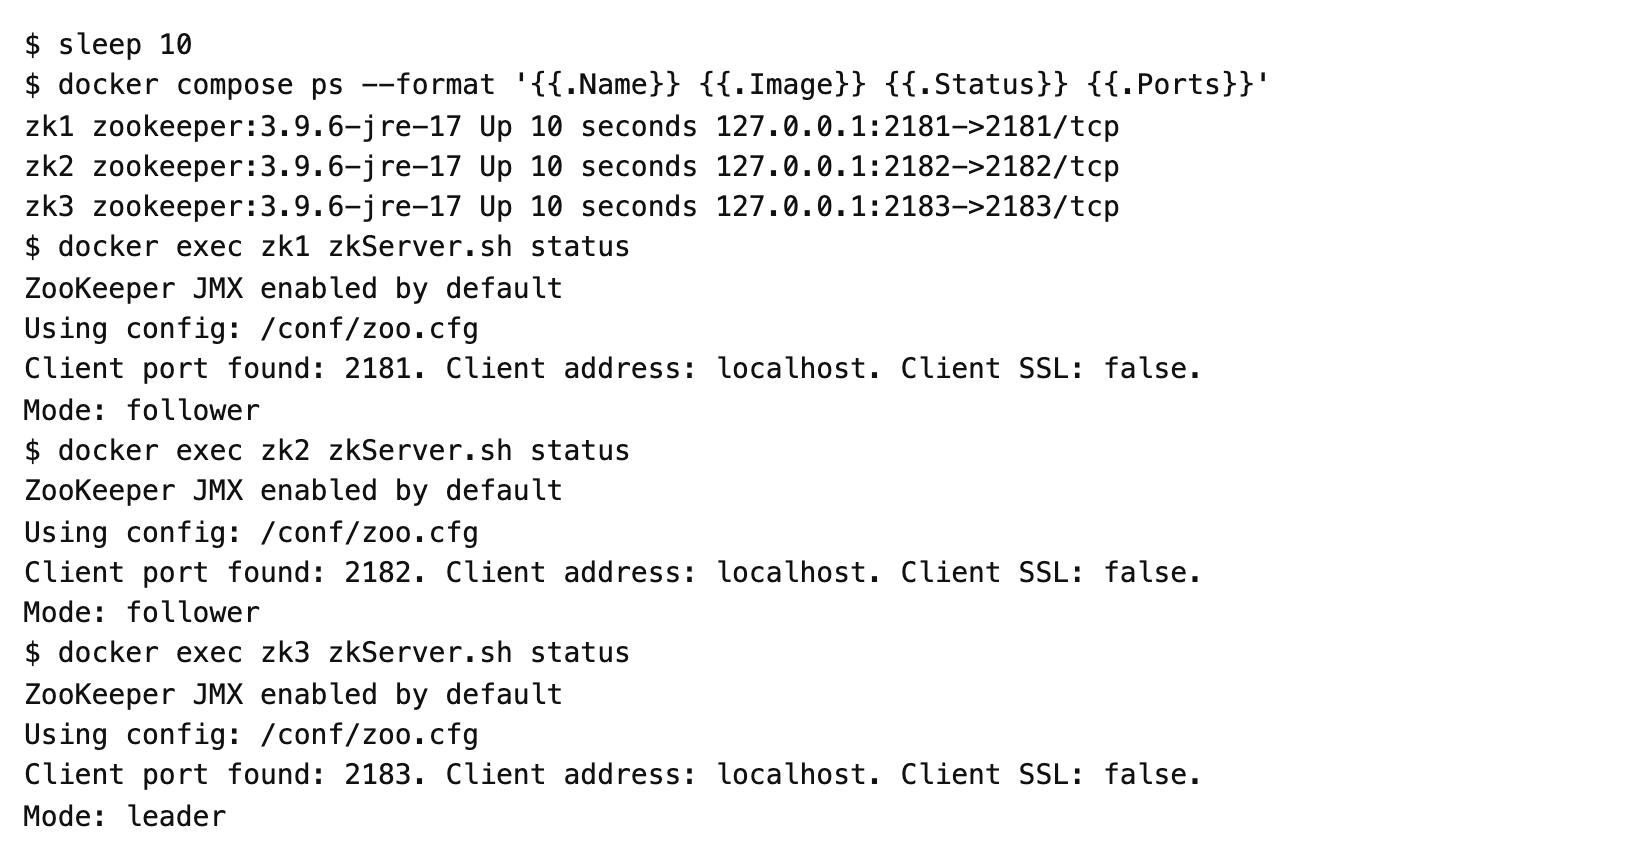
\includegraphics[width=0.85\textwidth,height=0.78\textheight,keepaspectratio]{../screenshots/02_roles.png}
\caption{Роли серверов после запуска}
\end{figure}

Затем остановлен лидер zk3. Через 5 секунд статус оставшихся серверов
показал нового лидера zk2, а zk1 остался последователем. Через zk1 создан узел
/quorum-check, через zk2 он прочитан. Два сервера из трех составляют
большинство, поэтому ансамбль продолжает принимать запись и чтение.

После остановки второго сервера zk1 работает один zk2. Его статус Error
contacting service, команда srvr отвечает This ZooKeeper instance is not
currently serving requests, а zkCli на запрос ls / получает ConnectionLoss.
Один сервер из трех не образует большинства, поэтому ансамбль не отвечает.
После запуска zk3 и zk1 все три сервера снова в ансамбле, лидер zk2, а узел
/quorum-check сохранился.

\begin{figure}[H]
\centering
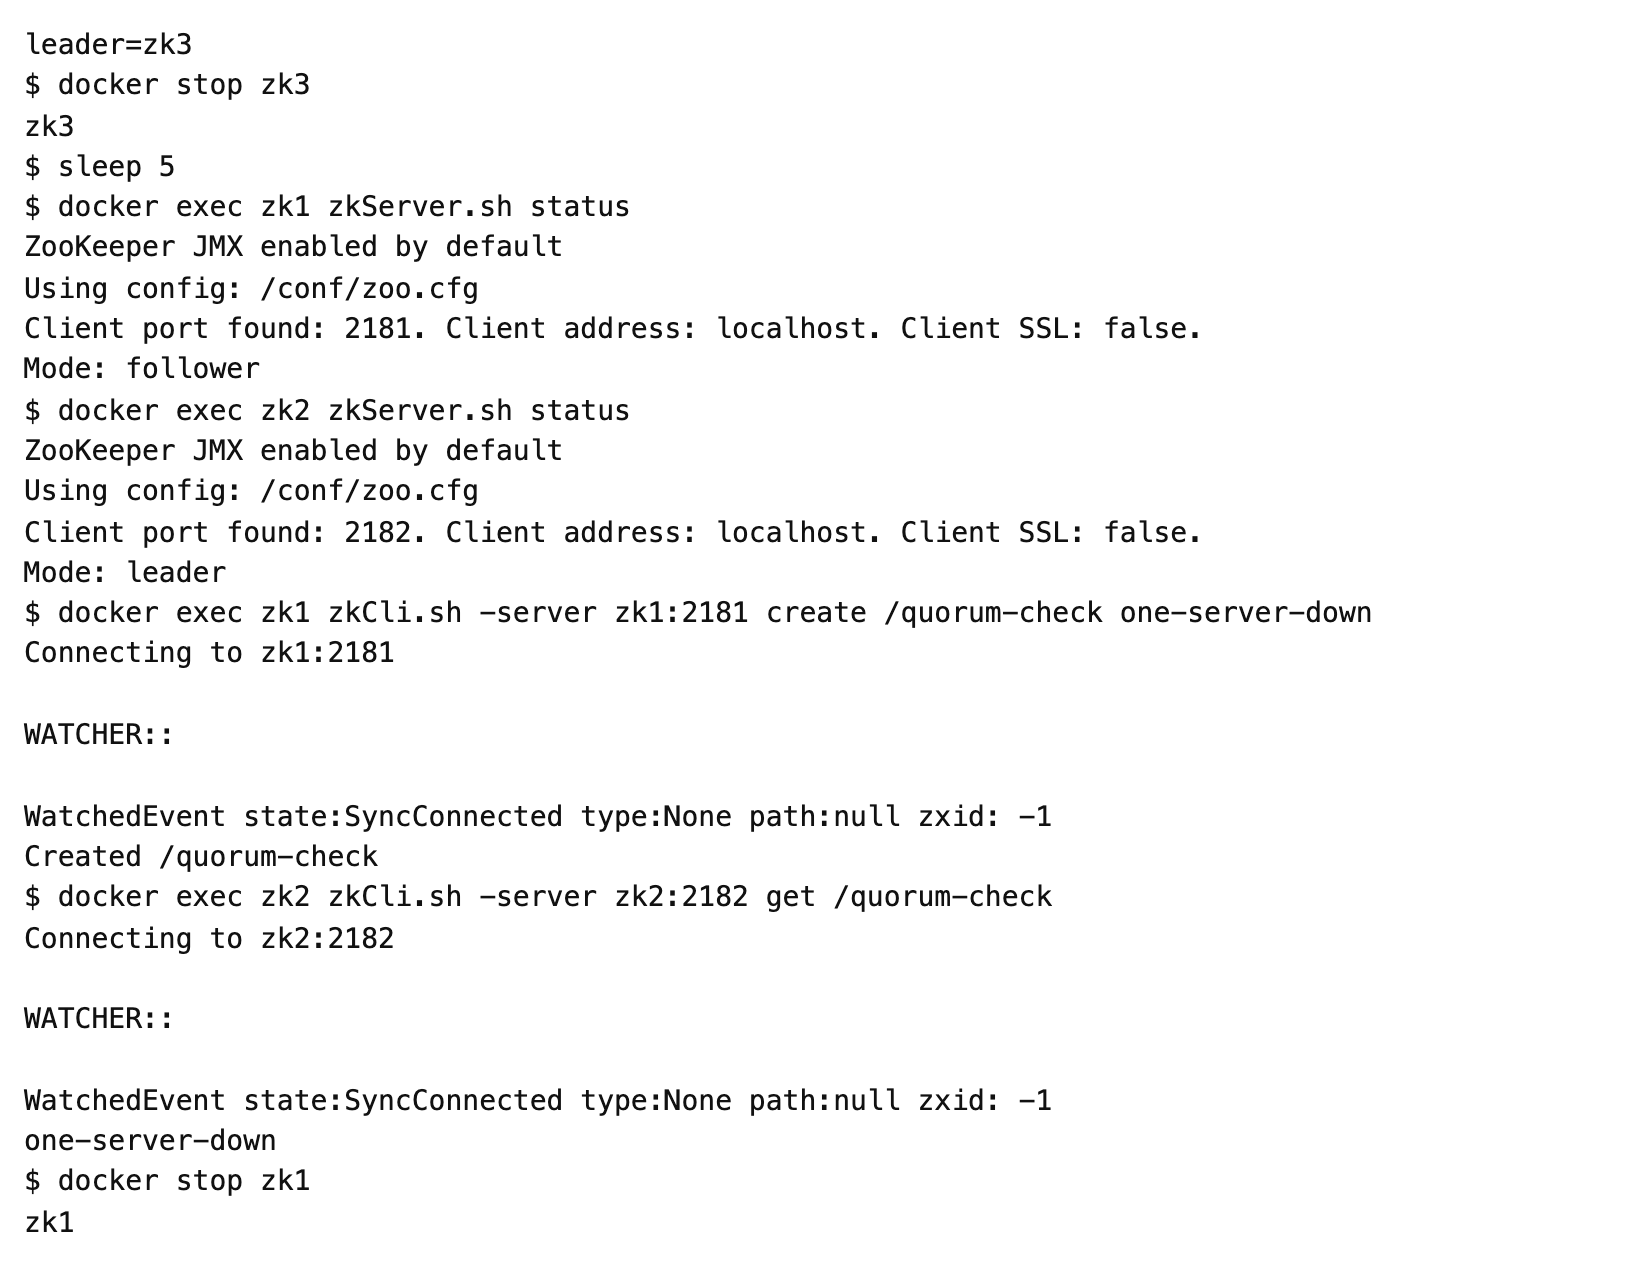
\includegraphics[width=0.85\textwidth,height=0.78\textheight,keepaspectratio]{../screenshots/03_quorum_1.png}
\caption{Потеря одного и двух серверов и возврат, часть 1 из 3}
\end{figure}

\begin{figure}[H]
\centering
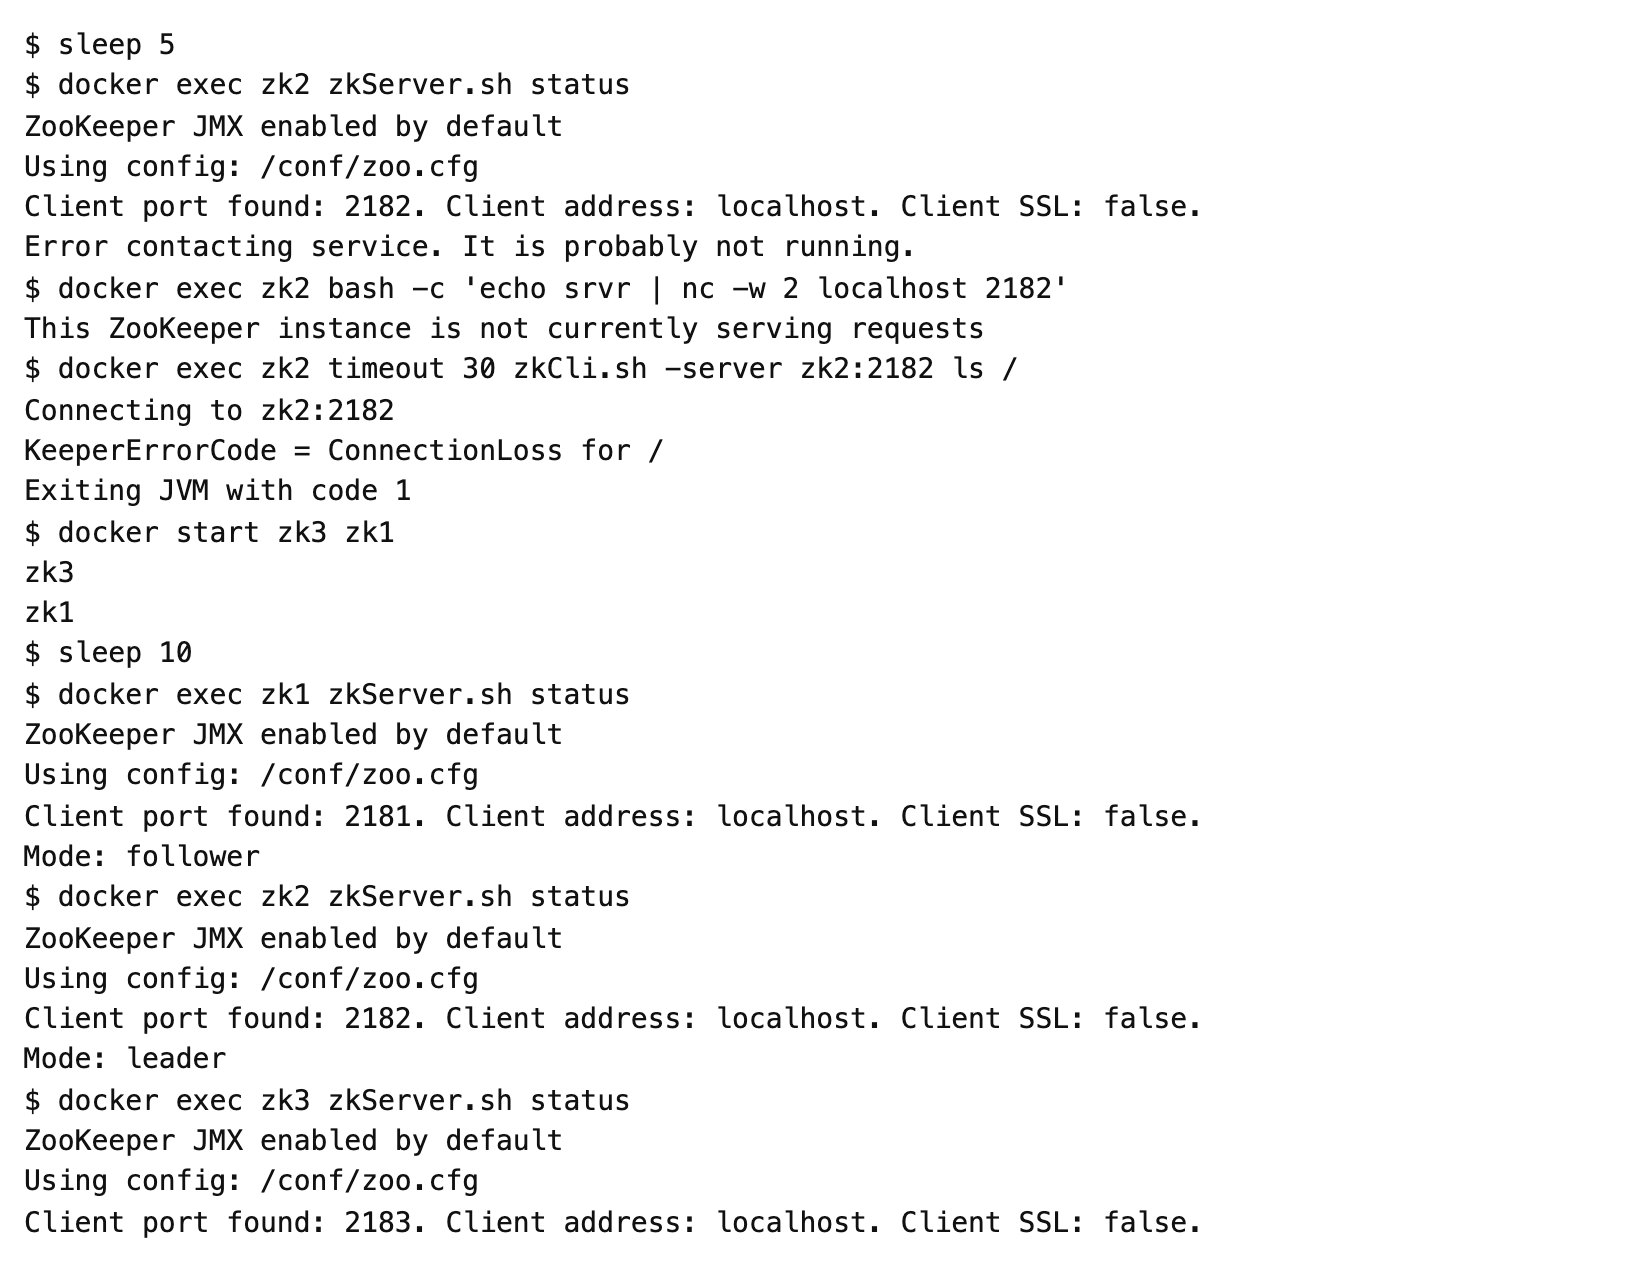
\includegraphics[width=0.85\textwidth,height=0.78\textheight,keepaspectratio]{../screenshots/03_quorum_2.png}
\caption{Потеря одного и двух серверов и возврат, часть 2 из 3}
\end{figure}

\begin{figure}[H]
\centering
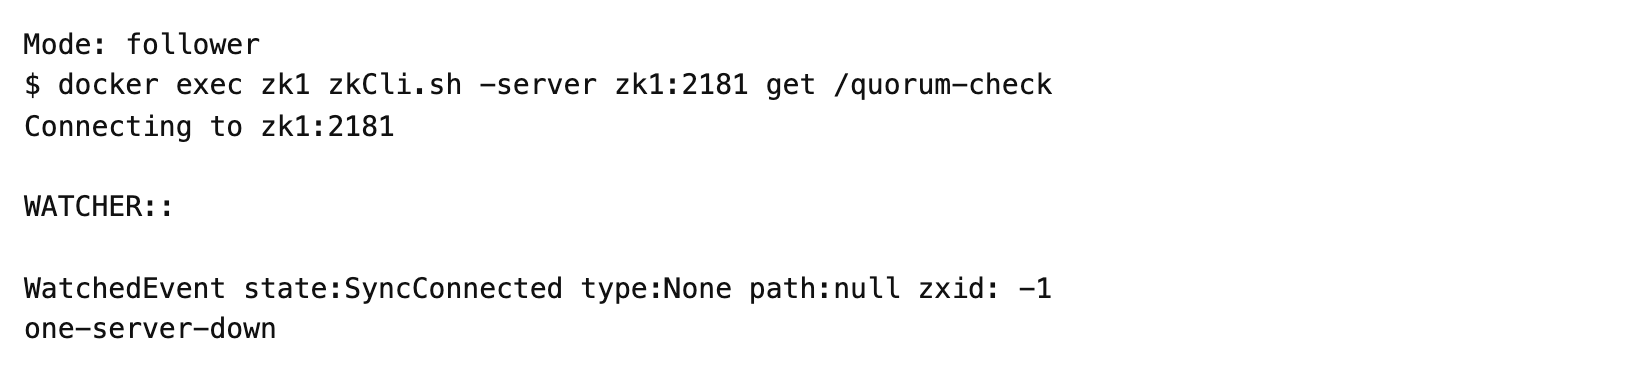
\includegraphics[width=0.85\textwidth,height=0.78\textheight,keepaspectratio]{../screenshots/03_quorum_3.png}
\caption{Потеря одного и двух серверов и возврат, часть 3 из 3}
\end{figure}

Эфемерный узел проверен двумя клиентами. Во втором окне zkCli создал узел
командой create -e /lab4-ephemeral и остался открытым. Из первого окна узел
виден, его поле ephemeralOwner равно 0x200000a87b40000, это номер сессии
второго окна. Затем второе окно закрыто, процесс клиента завершен сигналом
KILL, как при закрытии терминала. Клиент не успевает закрыть сессию сам,
поэтому сервер ждет истечения ее таймаута. Сессия zkCli по умолчанию
получает таймаут 30000 мс, это видно в обычном журнале клиента, а отсчет идет
от последнего сигнала клиента. Узел исчез
через 29 секунд после закрытия окна.

\begin{figure}[H]
\centering
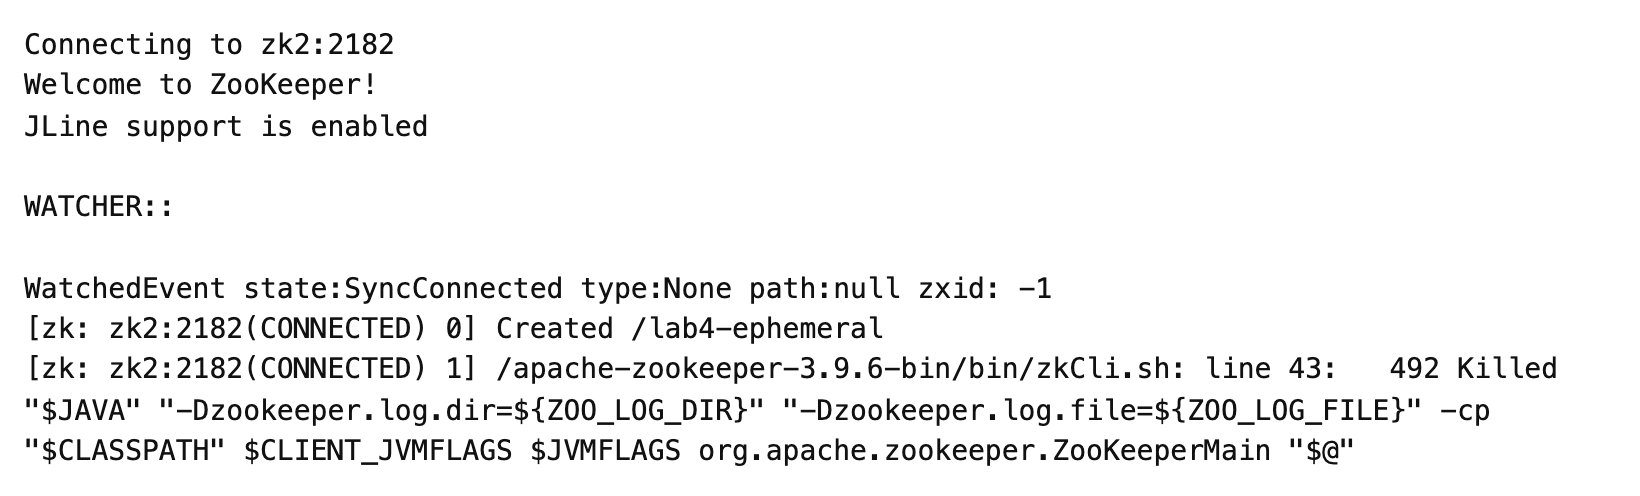
\includegraphics[width=0.85\textwidth,height=0.78\textheight,keepaspectratio]{../screenshots/04_ephemeral_window2.png}
\caption{Второе окно, создание эфемерного узла и закрытие клиента}
\end{figure}

\begin{figure}[H]
\centering
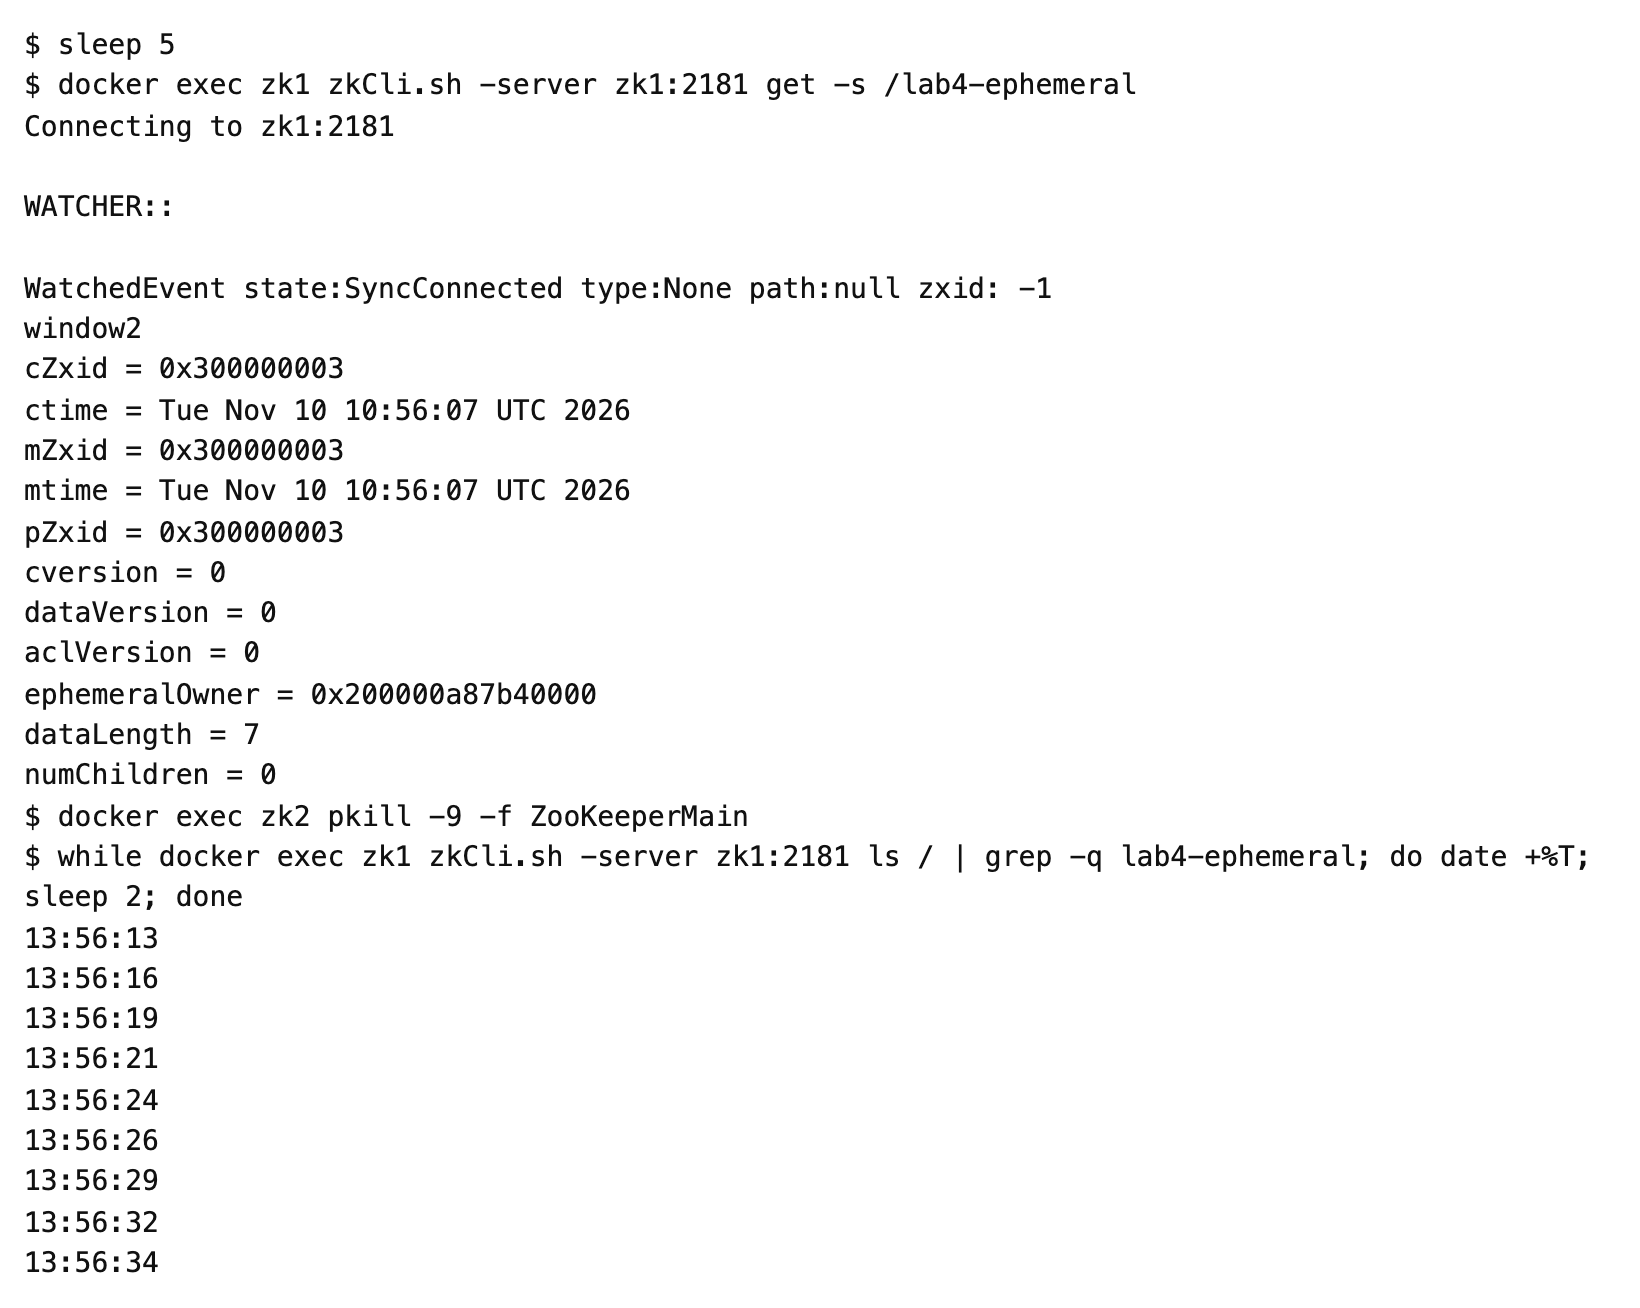
\includegraphics[width=0.85\textwidth,height=0.78\textheight,keepaspectratio]{../screenshots/04_ephemeral_window1_1.png}
\caption{Первое окно, узел виден, а после закрытия второго окна исчезает, часть 1 из 2}
\end{figure}

\begin{figure}[H]
\centering
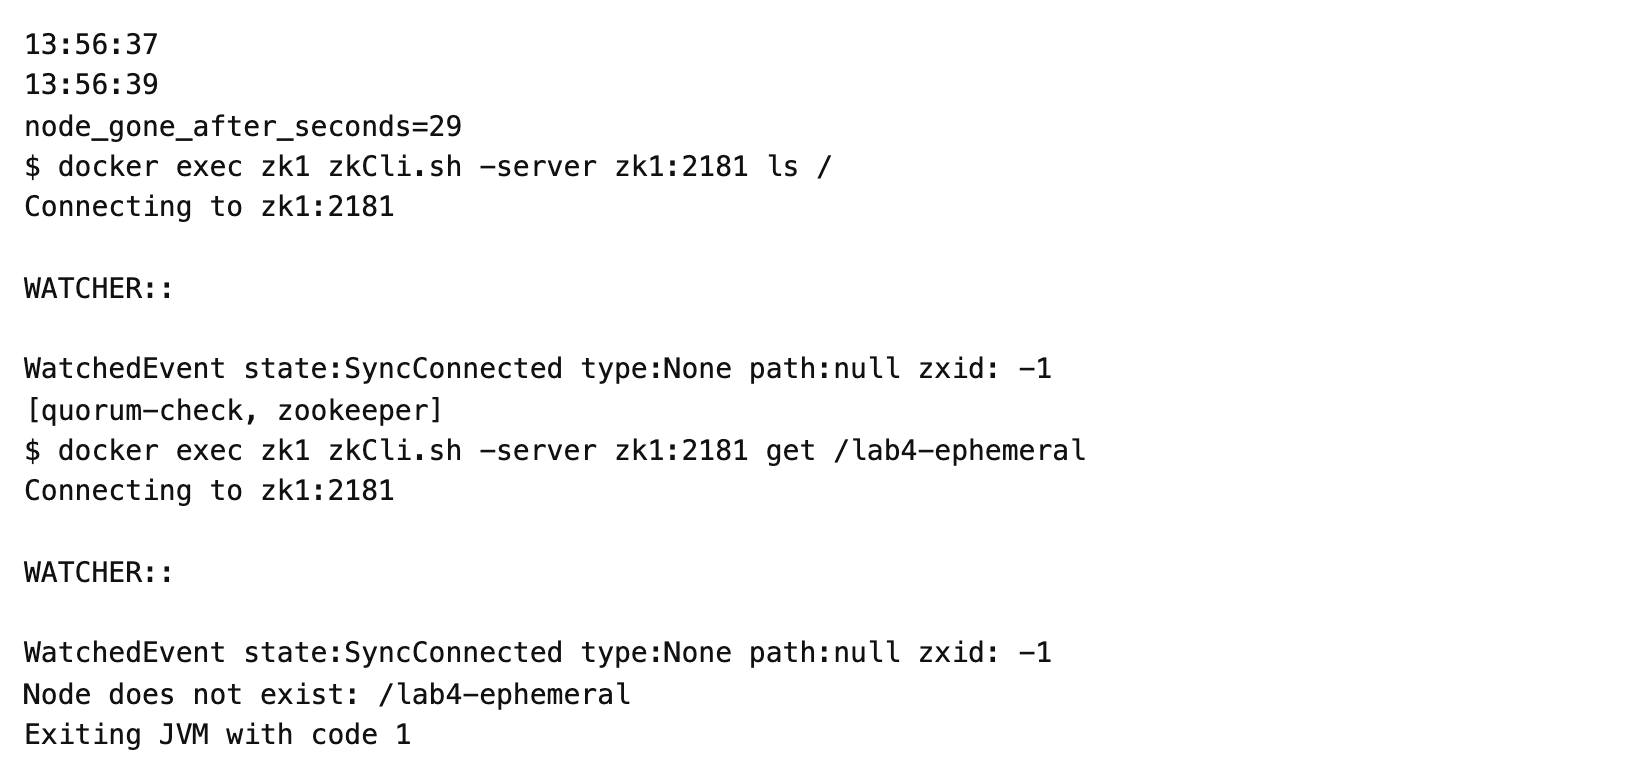
\includegraphics[width=0.85\textwidth,height=0.78\textheight,keepaspectratio]{../screenshots/04_ephemeral_window1_2.png}
\caption{Первое окно, узел виден, а после закрытия второго окна исчезает, часть 2 из 2}
\end{figure}

\section{3. Координатор расчета}

Координатор написан на Python с клиентом kazoo поверх расчета пар навыков
из третьей работы. Расчет тот же. Входной объект
s3://hh-lake/raw/it\_vacancies\_2024.csv лежит в RustFS из третьей работы,
условие варианта и нормализация навыков не изменились, объект делится на 26
сплитов по 32 МиБ. Сплиты обрабатывает лидер, а ZooKeeper хранит общее
состояние. Таймаут сессии клиента 10 секунд, сервер согласовал 10000 мс.

В ZooKeeper используются четыре узла. В \texttt{/lab4/election} кандидаты
создают эфемерные последовательные узлы. Кандидат с наименьшим номером
становится лидером, остальные ставят watch только на предыдущий узел, чтобы
не будить всех сразу. Когда сессия лидера истекает, его узел удаляется,
watch срабатывает, и лидером становится следующий кандидат.

Узел \texttt{/lab4/epoch} хранит номер эпохи. Новый лидер увеличивает его
условной записью по версии, поэтому у каждого лидера своя эпоха, у первого
1, у второго 2. Узел \texttt{/lab4/checkpoint} хранит список готовых
сплитов. После каждого сплита его пары сохраняются в бакет zk-lab, затем
номер сплита добавляется в чекпоинт. Новый лидер читает чекпоинт и
пропускает готовые сплиты. Когда готовы все 26 сплитов, лидер суммирует пары
и записывает файл результата в том же формате, что в третьей работе.

Узел \texttt{/lab4/result} это указатель на опубликованный результат. Без
защиты лидер записывает его безусловно. С FENCING=1 запись идет одной
транзакцией ZooKeeper. Транзакция проверяет, что версия узла эпохи осталась
той, которую лидер получил при избрании, и только тогда меняет указатель.
Если за это время избран другой лидер, проверка не проходит с
BadVersionError, и координатор удаляет свой неопубликованный файл.

\begin{code}
def wait_for_leadership(zk):
    me = zk.create(f'{ROOT}/election/n_', NAME.encode(), ephemeral=True, sequence=True)
    mine = me.rsplit('/', 1)[1]
    while True:
        kids = sorted(zk.get_children(f'{ROOT}/election'))
        idx = kids.index(mine)
        if idx == 0:
            return
        prev = f'{ROOT}/election/{kids[idx - 1]}'
        gone = threading.Event()
        if zk.exists(prev, watch=lambda event: gone.set()):
            gone.wait()

data, st = zk.get(f'{ROOT}/epoch')
epoch = int(data) + 1
epoch_version = zk.set(f'{ROOT}/epoch', str(epoch).encode(), version=st.version).version

if FENCING:
    tx = zk.transaction()
    tx.check(f'{ROOT}/epoch', epoch_version)
    tx.set_data(f'{ROOT}/result', pointer)
    res = tx.commit()
else:
    stat = zk.set(f'{ROOT}/result', pointer)
\end{code}

Запуски проводит скрипт scenario.py. Он сбрасывает узлы \texttt{/lab4},
запускает coord-a и coord-b, ждет, пока в чекпоинте наберется 8 сплитов из
26, и приостанавливает лидера сигналом SIGSTOP. Когда запасной координатор
записал результат, через 40 секунд после паузы лидер возобновляется сигналом
SIGCONT. В конце скрипт выводит время смены лидера, число записей
результата, указатель и сверку результатов с файлом пар из третьей работы по
SHA256. Каждый координатор пишет свой журнал в папку logs.

\section{4. Приостановка лидера без защиты}

Лидером стал coord-a с эпохой 1. После 8 сплитов он приостановлен в
13:59:16.925. В 13:59:28.184 coord-b стал лидером с эпохой 2, лидер сменился
через 11,26 секунды. Coord-b прочитал чекпоинт с 8 готовыми сплитами из 26,
продолжил со сплита 8, закончил расчет и записал результат, указатель
получил версию 1.

В 13:59:56.930 coord-a возобновлен. Его журнал показывает, что соединение
разорвано, сессия истекла и создана новая. Сам coord-a не узнал, что
лидером уже другой координатор. Он продолжил свои сплиты, закончил расчет и
в 14:00:01.902 записал результат второй раз, указатель получил версию 2 и
теперь указывает на файл coord-a. В журналах две строки записал результат.

Оба результата совпали с третьей работой. В каждом 12308 пар, сумма 48175,
первая пара android + kotlin в 784 вакансиях, SHA256 2fbb0cb56c472f16 такой
же, как у файла skills\_k2.csv из третьей работы. Здесь повторная запись
ничего не испортила только потому, что результаты одинаковые. Если бы
старый лидер посчитал по устаревшим данным, он перезаписал бы правильный
результат.

Время смены лидера складывается из таймаута сессии 10 секунд и шага, с
которым сервер проверяет истекшие сессии. Этот шаг равен tickTime, 2
секунды, поэтому сессия истекает через 10 до 12 секунд после последнего
запроса клиента. Удаление узла кандидата и срабатывание watch занимают
миллисекунды.

\begin{figure}[H]
\centering
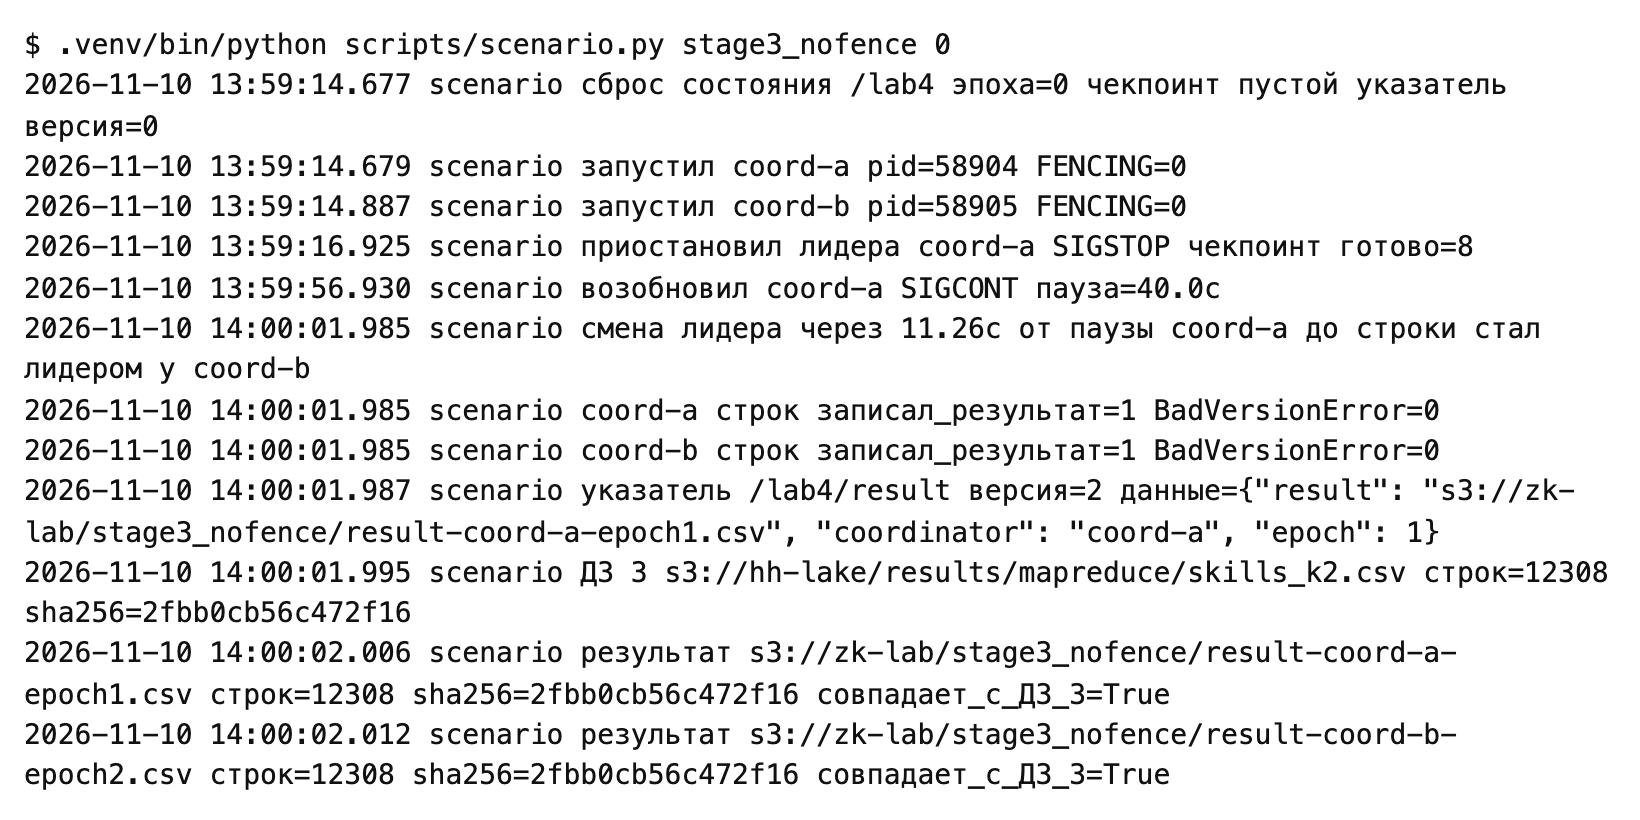
\includegraphics[width=0.85\textwidth,height=0.78\textheight,keepaspectratio]{../screenshots/stage3_nofence_scenario.png}
\caption{Этап 3, итог сценария без защиты}
\end{figure}

\begin{figure}[H]
\centering
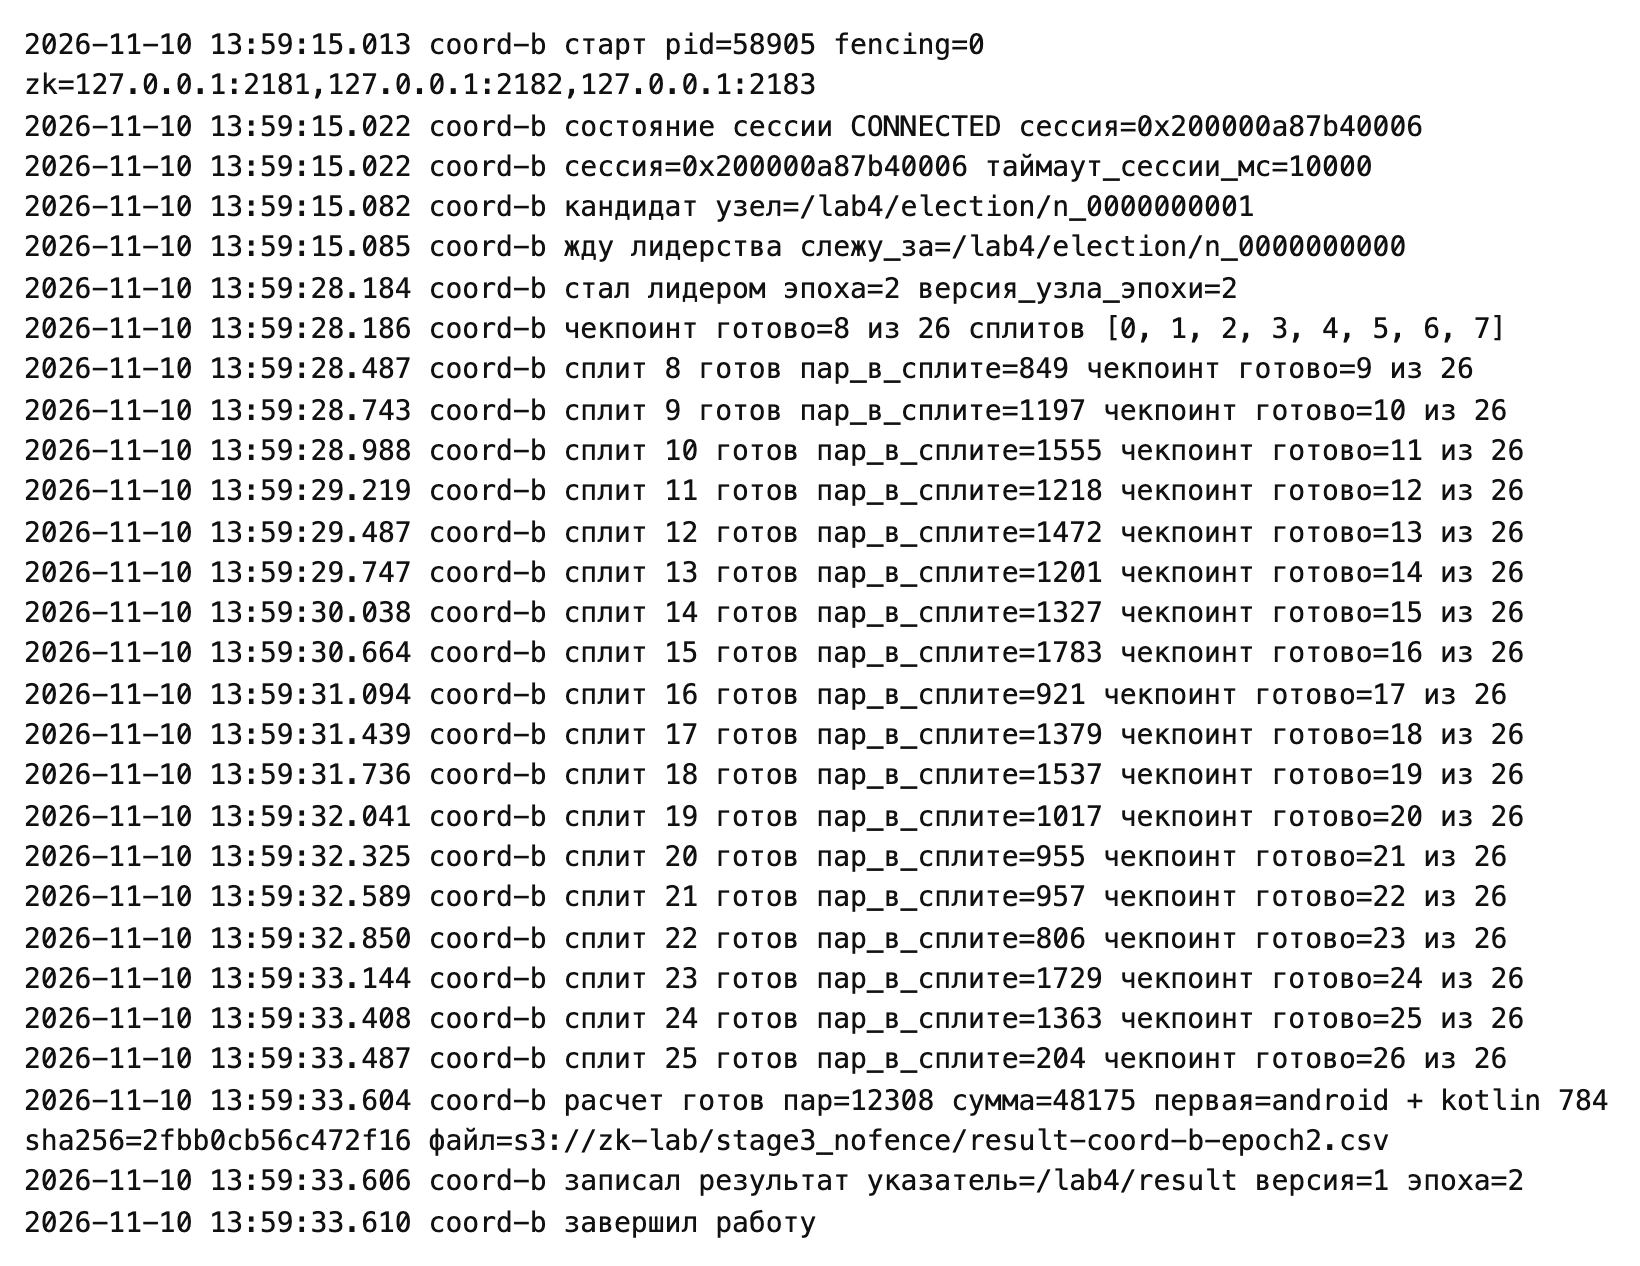
\includegraphics[width=0.85\textwidth,height=0.78\textheight,keepaspectratio]{../screenshots/stage3_nofence_coord-b.png}
\caption{Этап 3, журнал запасного координатора coord-b}
\end{figure}

\begin{figure}[H]
\centering
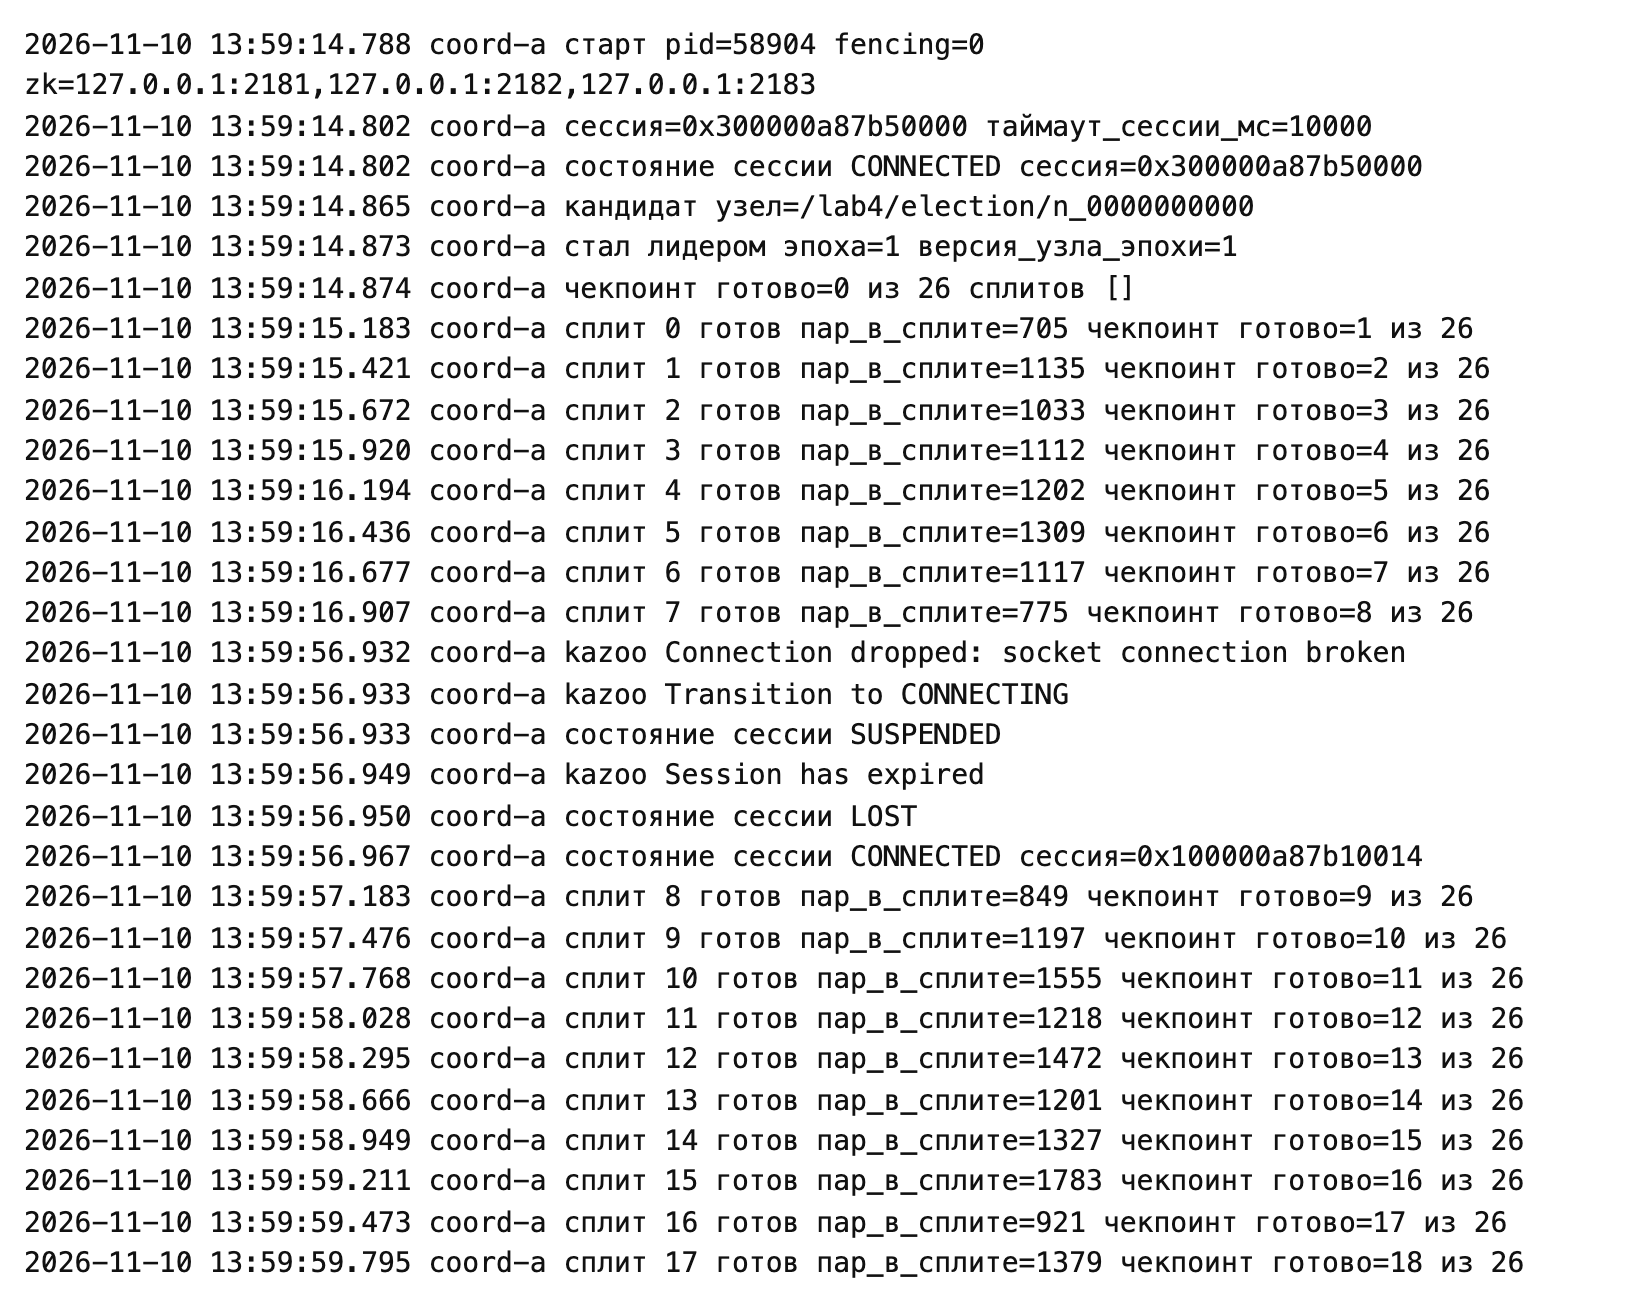
\includegraphics[width=0.85\textwidth,height=0.78\textheight,keepaspectratio]{../screenshots/stage3_nofence_coord-a_1.png}
\caption{Этап 3, журнал приостановленного лидера coord-a, часть 1 из 2}
\end{figure}

\begin{figure}[H]
\centering
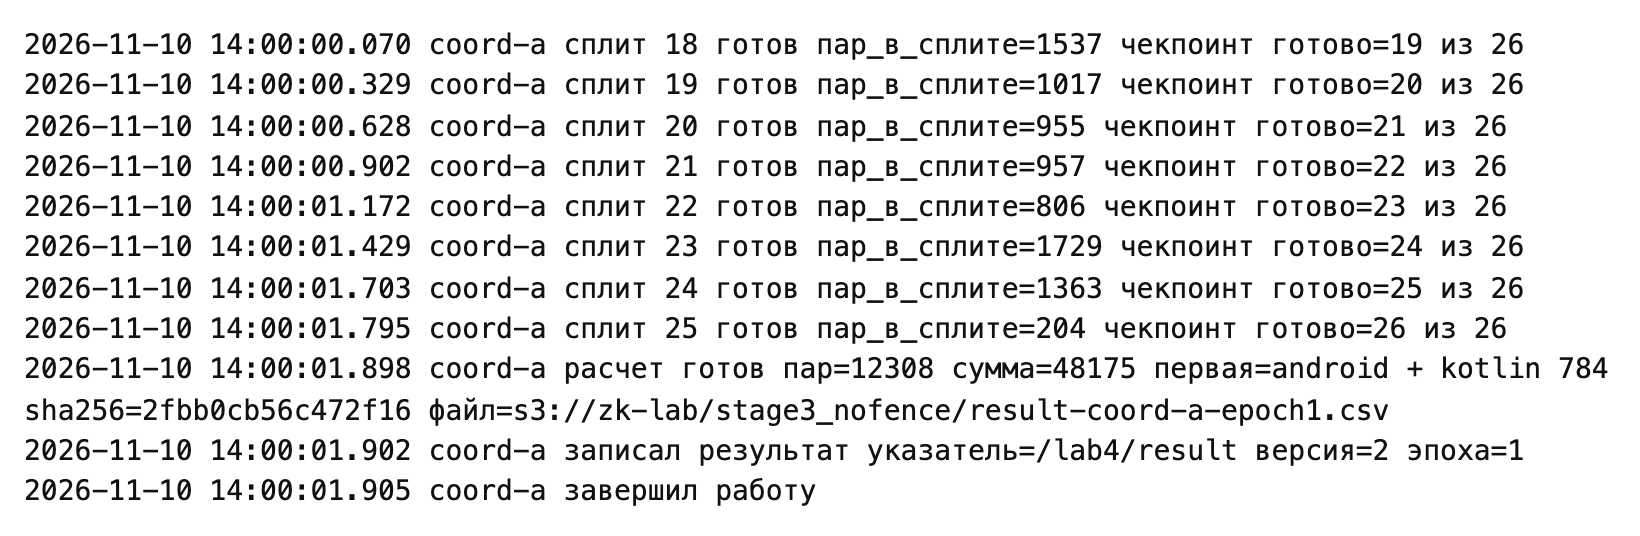
\includegraphics[width=0.85\textwidth,height=0.78\textheight,keepaspectratio]{../screenshots/stage3_nofence_coord-a_2.png}
\caption{Этап 3, журнал приостановленного лидера coord-a, часть 2 из 2}
\end{figure}

\section{5. Приостановка лидера с защитой по эпохе}

Запуск повторен с FENCING=1. Coord-a с эпохой 1 приостановлен в
14:00:05.109 после 8 сплитов. В 14:00:16.184 coord-b стал лидером с эпохой 2,
лидер сменился через 11,08 секунды. Coord-b продолжил с чекпоинта и
транзакцией записал указатель версии 1.

После возобновления coord-a снова досчитал результат, его SHA256 тоже
2fbb0cb56c472f16. Транзакция coord-a проверяла версию узла эпохи, полученную
при его избрании, а эпоха уже была 2. Запись отклонена с BadVersionError,
coord-a удалил свой неопубликованный файл. Указатель остался версии 1 от
coord-b, в бакете один результат, и он совпадает с третьей работой.

\begin{figure}[H]
\centering
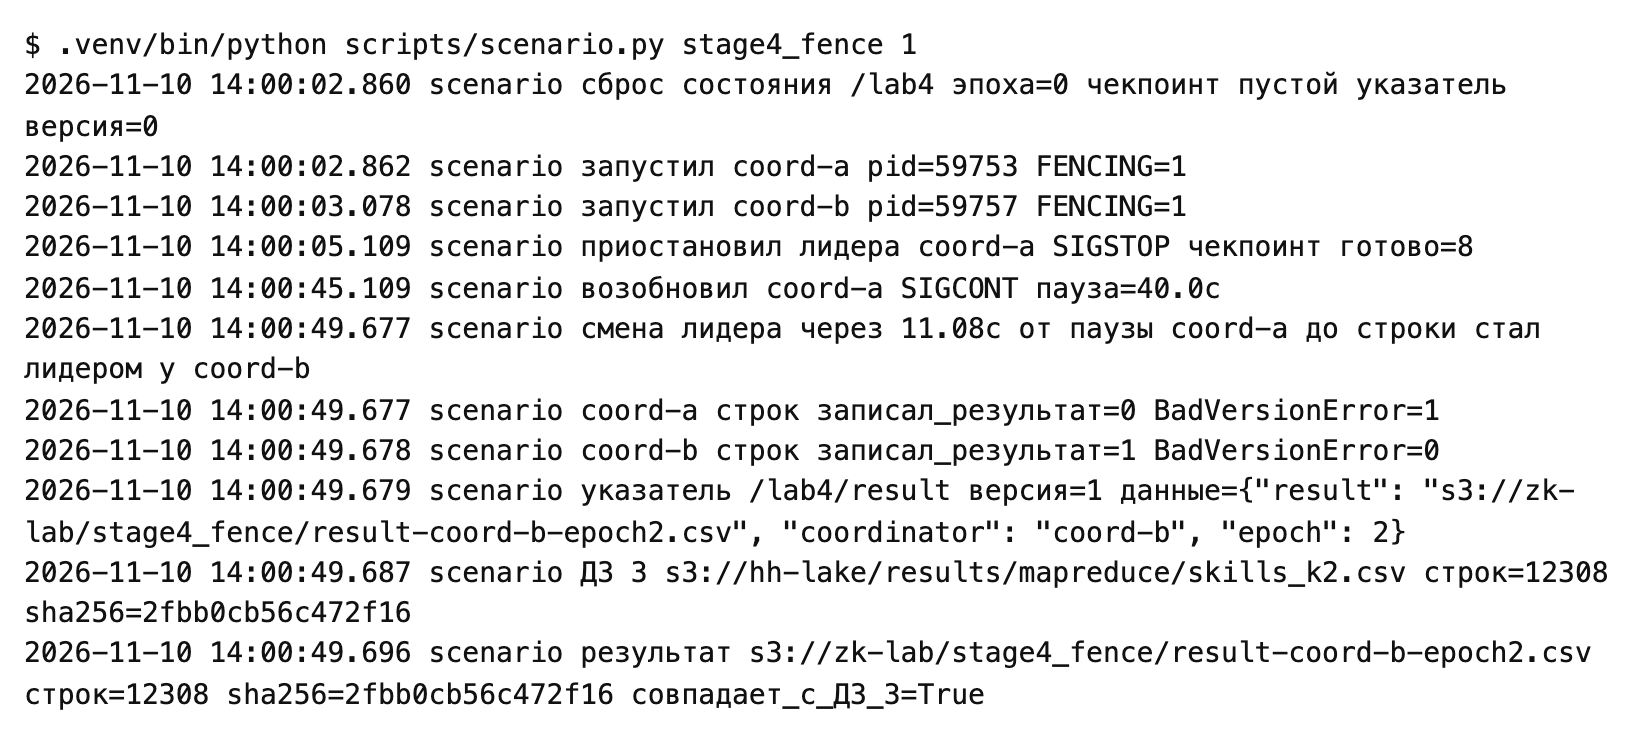
\includegraphics[width=0.85\textwidth,height=0.78\textheight,keepaspectratio]{../screenshots/stage4_fence_scenario.png}
\caption{Этап 4, итог сценария с защитой по эпохе}
\end{figure}

\begin{figure}[H]
\centering
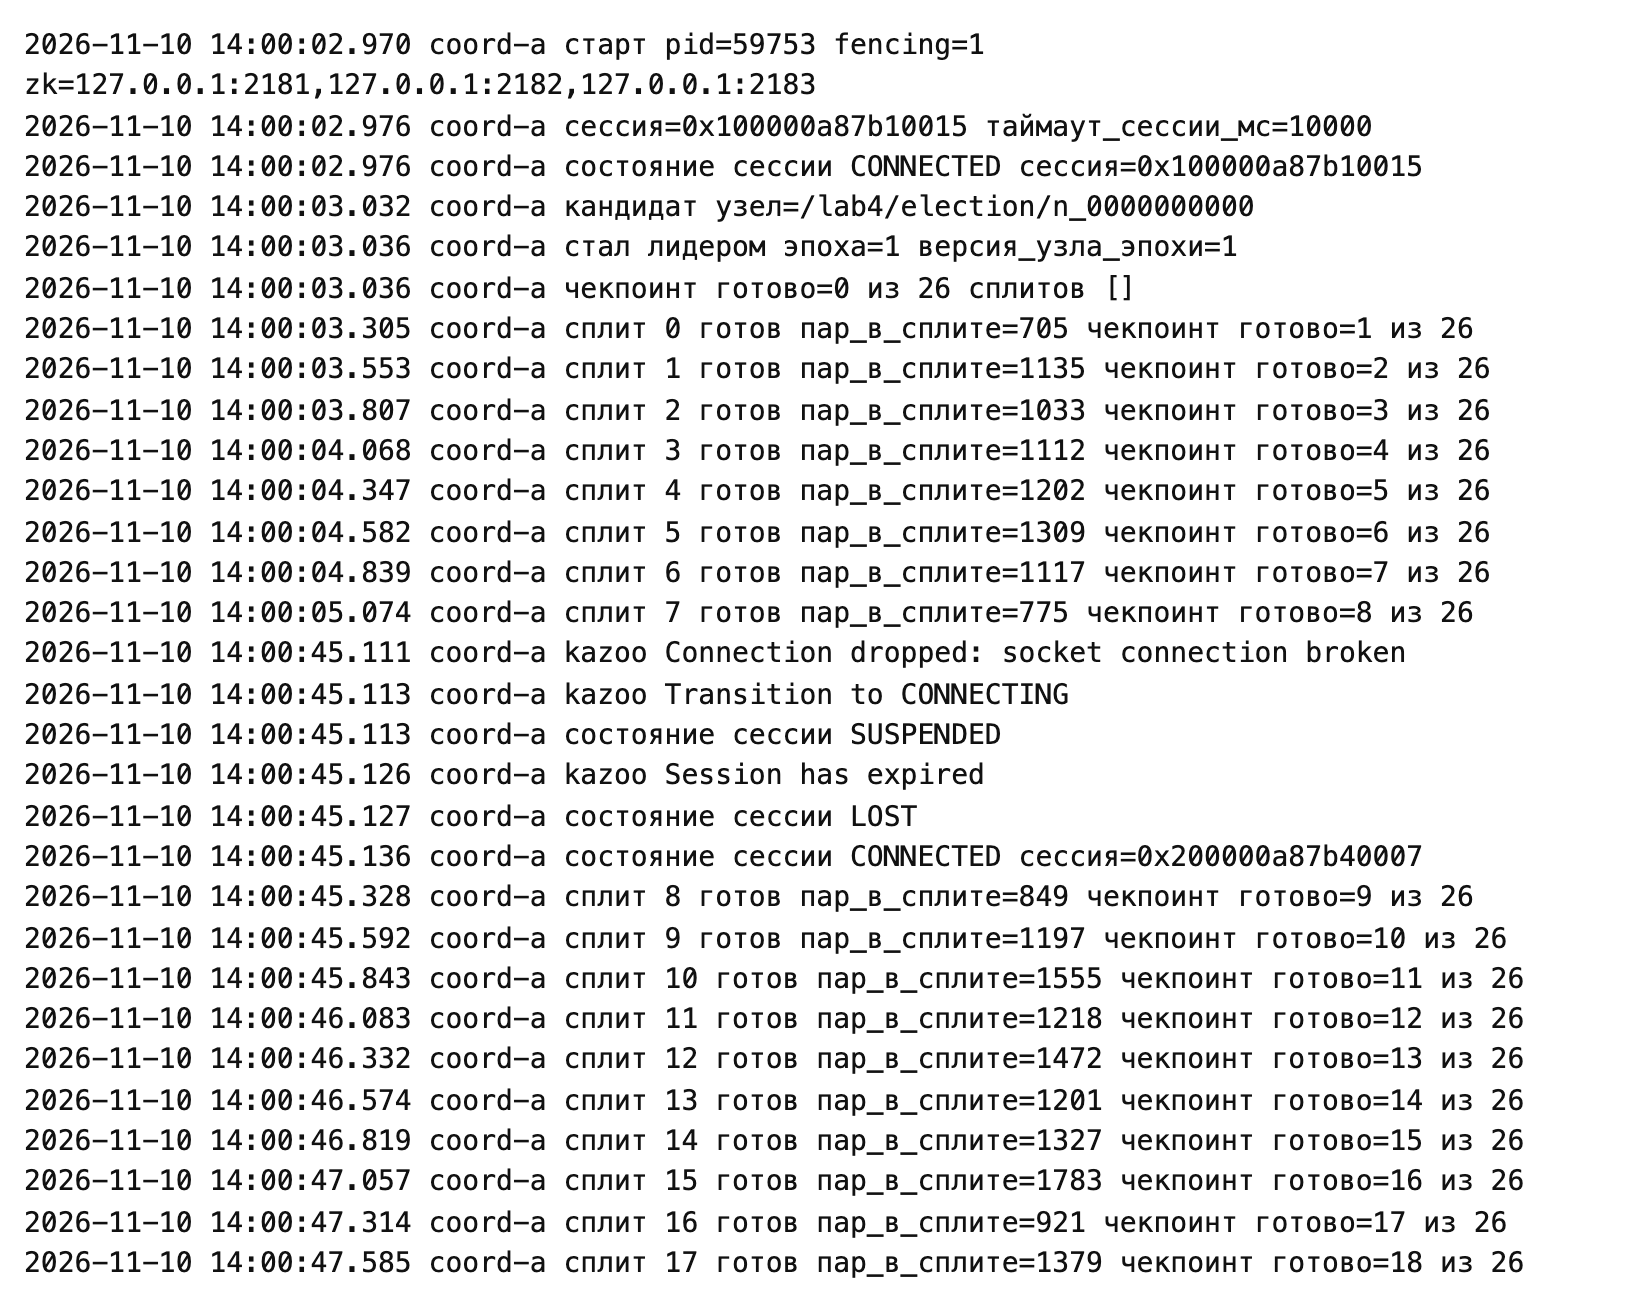
\includegraphics[width=0.85\textwidth,height=0.78\textheight,keepaspectratio]{../screenshots/stage4_fence_coord-a_1.png}
\caption{Этап 4, журнал coord-a с отклоненной записью, часть 1 из 2}
\end{figure}

\begin{figure}[H]
\centering
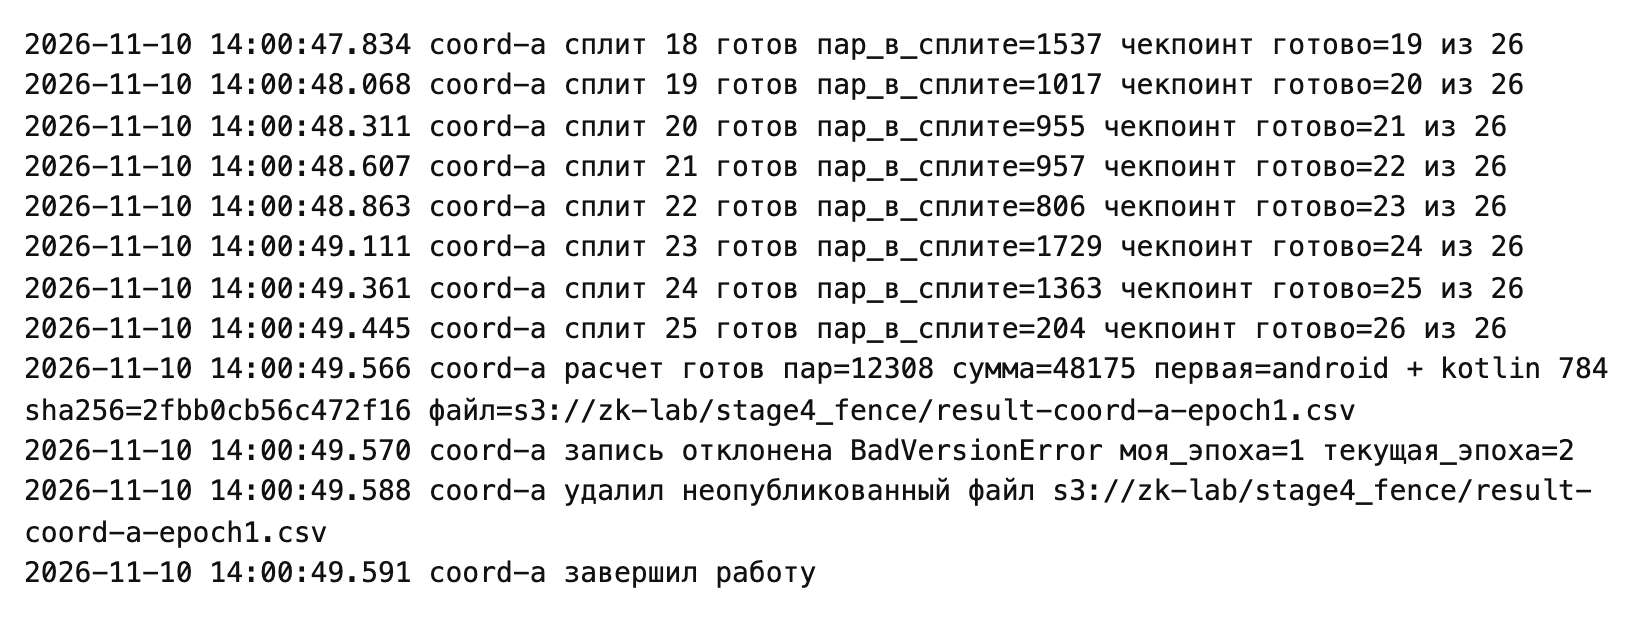
\includegraphics[width=0.85\textwidth,height=0.78\textheight,keepaspectratio]{../screenshots/stage4_fence_coord-a_2.png}
\caption{Этап 4, журнал coord-a с отклоненной записью, часть 2 из 2}
\end{figure}

\begin{figure}[H]
\centering
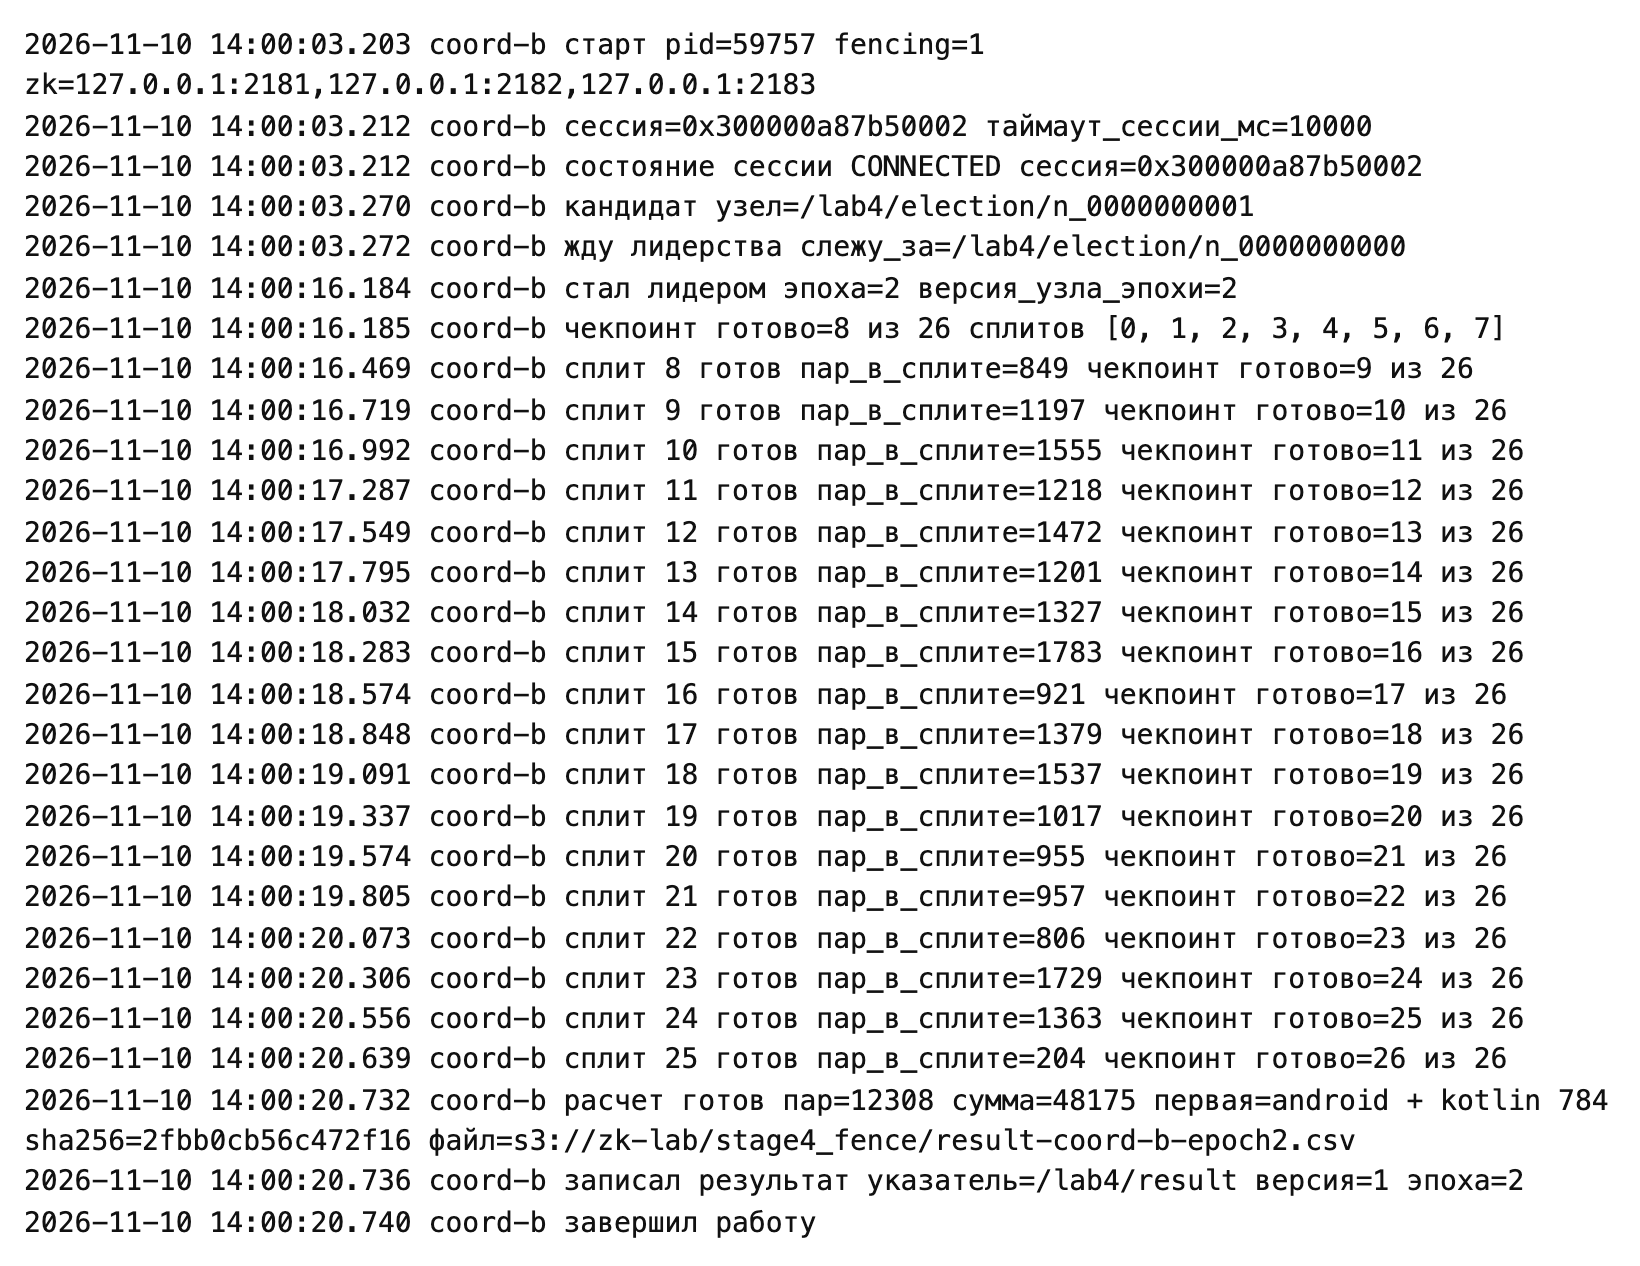
\includegraphics[width=0.85\textwidth,height=0.78\textheight,keepaspectratio]{../screenshots/stage4_fence_coord-b.png}
\caption{Этап 4, журнал coord-b}
\end{figure}

\section{6. Ответы на вопросы}

Почему серверов три, а не два и не четыре. Ансамбль работает, пока живо
большинство серверов. Из двух серверов большинство это оба, и отказ любого
останавливает сервис, то есть второй сервер добавляет еще одну точку отказа
и не дает устойчивости. Из трех серверов большинство это два, поэтому один
сервер можно потерять. Это видно в работе, без zk3 ансамбль принимал запись,
а без двух серверов перестал отвечать. Четыре сервера тоже переживают отказ
только одного, потому что большинство из четырех это три. При этом запись
ждет подтверждения от трех серверов вместо двух, а машин больше. Кроме
того, при разрыве сети пополам два на два ни одна половина не получит
большинства. Поэтому число серверов берут нечетным, и три это наименьший
ансамбль, который переживает отказ одного сервера.

Почему защиту по эпохе проверяет получатель записи, а не ZooKeeper.
ZooKeeper знает только о сессиях и узлах. Он заметил, что сессия coord-a
истекла, удалил его узел и дал лидерство coord-b. Но остановить
приостановленный процесс или забрать у него уже начатую работу ZooKeeper не
может. Проснувшийся coord-a считал себя лидером и сразу пошел записывать
результат. Проверка самим лидером перед записью тоже не спасает, потому что
пауза может случиться между проверкой и записью. Отличить старую запись от
новой может только тот, кто применяет запись, ведь он видит все записи по
порядку и знает последнюю эпоху. Поэтому эпоха передается вместе с записью,
а получатель сравнивает ее с текущей и отклоняет устаревшую. У нас получатель
это узел указателя, и сравнение делает транзакция в момент записи, в журнале
это строка с BadVersionError. Если бы результат публиковался в базу данных
или в хранилище, хранить последнюю эпоху и проверять ее пришлось бы им, а
механизм лидерства ZooKeeper здесь ничем бы не помог.

Конфигурации серверов, compose.yaml, код координатора, журналы всех запусков,
выводы команд и этот отчет опубликованы в репозитории
\url{https://github.com/Gegerout/data-engineering-lab4}.
